\documentclass[conference]{IEEEtran}
\IEEEoverridecommandlockouts
% The preceding line is only needed to identify funding in the first footnote. If that is unneeded, please comment it out.
\usepackage{cite}
\usepackage{amsmath,amssymb,amsfonts}
\usepackage{algorithmic}
\usepackage{graphicx}
\usepackage{textcomp}
\usepackage{xcolor}
\usepackage{hyperref}
\usepackage{lipsum}
\DeclareMathOperator*{\argmin}{arg\,min}

\def\BibTeX{{\rm B\kern-.05em{\sc i\kern-.025em b}\kern-.08em
    T\kern-.1667em\lower.7ex\hbox{E}\kern-.125emX}}
\begin{document}

\title{Atlas based segmentation consists of a powerful baseline for brain tissue segmentation when compared to an ML based approach}

\author{\IEEEauthorblockN{Cyril Albrecht}
\and
\IEEEauthorblockN{Valerio Mollet}
\and
\IEEEauthorblockN{Quentin Savary}
}

\maketitle

\begin{abstract}
Medical image analysis usually uses atlas-based methods to segment brain tissues. Machine learning based methods could replace those older ones in the near future. Both types of segmentation have been compared, as well as the influence of affine or non-rigid registration before-hand. Only five tissues of the brain have been been segmented with 20 training images and 10 test images. The results are compared with the Dice score and Hausdorff distance.

Atlas-based segmentations give better results with smaller brain parts (amygdala, hippocampus, and thalamus). Geometrically complex parts (grey and white matter) have better results when segmented with a machine learning method. The best overall solution is obtained with a locally weighted atlas-based segmentation.
\end{abstract}

\begin{IEEEkeywords}
% needed?
\end{IEEEkeywords}

% 
\section*{Introduction}
Medical images are widely used for all kinds of diagnoses such as tumour detection and tissue segmentation. Those are tedious and repetitive tasks for the medical personnel. A medical image analysis (MIA) pipeline is a tool that can reduce the time needed to perform said tasks. The current trend of machine learning offers new possibilities for this tool, especially in the classification step.
In this project, the hypothesis was made that Atlas based segmentation consists of a powerful baseline for brain tissue segmentation when compared to an ML based approach. To accept or reject this hypothesis, different atlas-based segmentations were implemented and compared with machine learning.
In this project, four variations of atlas-based segmentation and a simple machine learning algorithm are compared. Those are majority voting, global and local weighted voting, shape based averaging, and random forest for the machine learning segmentation. The comparison is done with a Dice score and a Hausdorff distance, two widely used measurement tools. For simplicity, only five brain tissues have been segmented: grey and white matter, the amygdala, hippocampus, and thalamus. A total of 30 anonymized images have been used, 20 for training and 10 for testing. As it has quite some influence for segmentation, two kinds of registration have also been compared: affine and non-rigid.

\subsection*{Related work}
Organ segmentation is a big part of medical image processing, so there are very many methods to segment organs. The methods work better or worse depending on the organ to be segmented. The atlas based methods for segmentation are described in detail in different works and were adapted in this work. Here is a list of the papers we used to write the algorithms for this project:

\begin{itemize}
	\item Combination strategies in multi-atlas image segmentation: Application to brain MR data\cite{b2}
	\item Another entry in the list
\end{itemize}



\section*{Method}

\subsection*{MIA pipeline} \label{sec:MIApipeline}
The medical image analysis pipeline consists of five distinct steps: registration, pre-processing, feature extraction, classification and post-processing. It is illustrated in the Fig. \ref{fig:pipeline}.

\begin{figure}[h!]
	\centering
	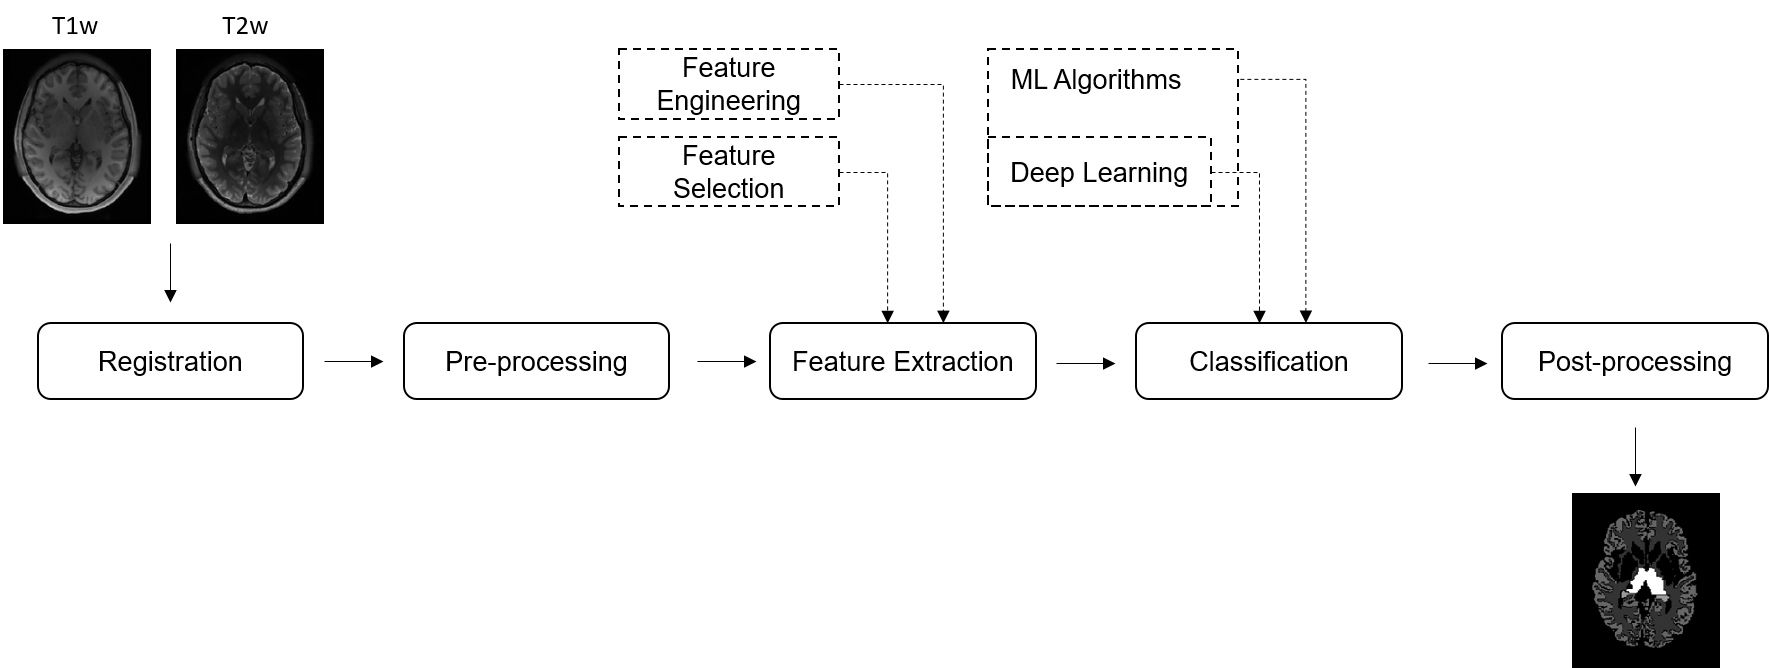
\includegraphics[width = .45 \textwidth]{img/pipeline}
	\caption{Schematic of the medical image analysis pipeline.}
	\label{fig:pipeline}
\end{figure}

Registration matches an acquired image to a reference one, usually provided from an atlas. This image transformation can be affine as well as non-rigid, which allows local deformations. The pre-processing is used to improve the quality of an image. It uses different kind of filters and masks to get a higher quality image or remove unnecessary data. Intensity normalization is also used, especially if machine learning is involved. Feature extraction tries to find position of anatomical landmarks. Contours and corners can be found with rather simple algorithms. Classification means to decide of the anatomical type for each voxel. This can be done in various ways, decisions trees (also called random forests) in machine learning or by growing regions algorithms. Finally, post-processing gives a cleaner final segmentation. It will remove small groups of voxels that should not correspond to any real anatomical part. As an example, a human body can only have one liver or two kidneys of similar size.

To measure the overall performance, several evaluation metrics can be used. The Dice coefficient tells how good the computed result and the ground truth do overlap. It goes from 0 if there is no overlap at all to 1 being exactly same segmentation. The Hausdorff distance is another metric. It measures the maximum distance from the computed segmentation contour to the ground truth one. There are many more metrics that can be used to test specific characteristics of a computed segmentation.

\subsection*{Registration}
For the registration step, two different solutions have been compared. The first is affine transformation, which which allows translation, rotation and scaling. The second one is non-rigid, which transforms the volumes locally. This can lead to a better matching between the input image and the atlas. For the affine registration of two volumes, the volume to be registered is moved relative to the fixed volume by rotation, translation or scaling. After each displacement a similarity of the volumes is measured. This parameter is minimized by moving the volume further until a minimum is reached. The same is true for a non rigid registration, but there is an additional tuning factor which allows local displacements, rotations and scaling. We used the \textit{Simple Elastix}\footnote{\url{https://github.com/SuperElastix/SimpleElastix}} library to compute the non-rigid transformation. This library uses a B-spline registration to register the two volumes non rigidly.

\subsection*{Segmentation}
For the segmentation step, a total of five methods have been compared. The first one is machine learning based, essentially a random forest with 10 estimators of maximum depth of 40. These parameters were found step by step with a manual optimization. For this, first one parameter was kept constant while the other was optimized and then vice versa. The other four methods were atlas-based, where mainly the weight function has been modified. The simplest one is when all images have the same weight. To reduce potentially worse ground truth inputs, we used global and local weights. In order to make the segmentation smoother, an additional method called Shape based averaging was implemented.

\subsubsection*{Machine Learning}
\subsubsection*{Majority Voting}

\begin{figure}[h!]
	\centering
	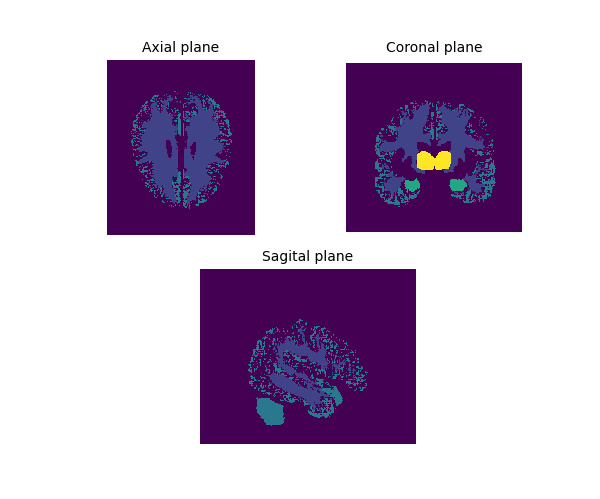
\includegraphics[width=0.8\linewidth]{img/majorityVoting}
	\caption{Schematic representation of majority voting.}
	\label{fig:majorityVoting}
\end{figure}

\subsubsection*{Global Weighted Voting}
Global weighted voting is an atlas-based segmentation method that takes into account individual variations of the target being segmented with the available atlases. Voting of atlases with high similarity to the target being segmented are weighted higher. In our case, the T1w and T2w volumes of 20 atlases were compared with the T1w and T2w volumes of the target. By measuring the mean square differences (MSD) averaged over both T1w and T2w volumes, each atlas was given a corresponding weight.  The weights were distributed by a soft maximization function so that the sum of all weights would equal one. This simplifies the calculation of the probability of the prediction. To get the segmentation, a majority voting is performed with the globally calculated weights.

\begin{figure}[h!]
	\centering
	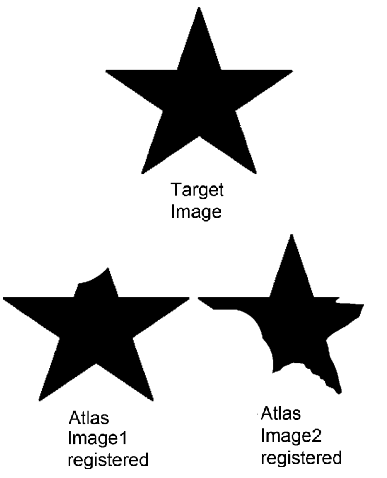
\includegraphics[width=0.5\linewidth]{img/globalWeightedProblematic}
	\caption{Example for showing the problem of global weighted voting. \color{red} Add reference Combination strategies in multi-atlas image segmentation: Application to brain MR data}
	\label{fig:globalweightedproblematic}
\end{figure}

The problem of this method is that an atlas is very similar in most parts but local is very different compared to the target. The weighting is still high due to the overall similarity. The opposite can also be the case, so that the overall similarity is very low but the atlas still has a very high correlation with the target in local parts. Thus, this similarity is not accounted for by the global weighting. To give this local similarities weighting, a local weighted voting can be performed. This problem is well illustrated in Fig. \ref{fig:globalweightedproblematic}.

\subsubsection*{Local Weighted Voting}

\begin{figure}[h!]
	\centering
	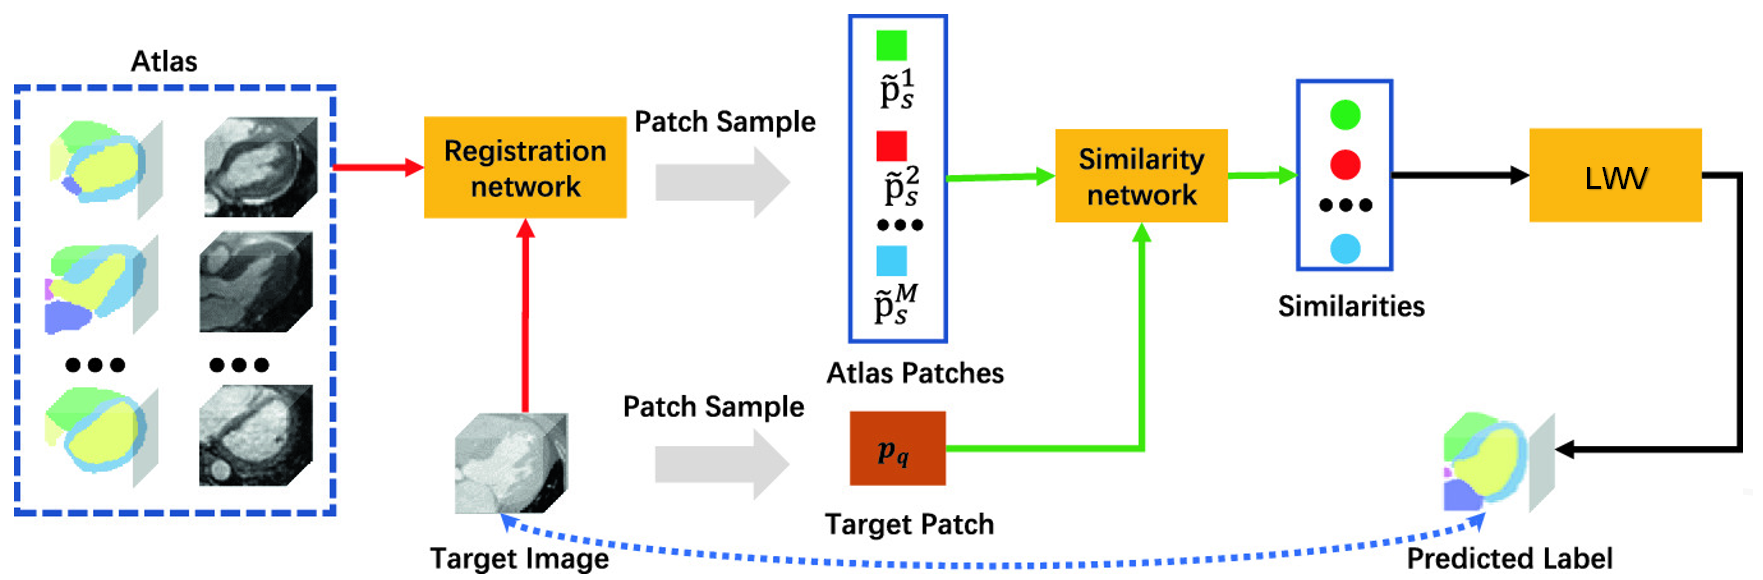
\includegraphics[width=0.8\linewidth]{img/localWeightedVoting}
	\caption{Schematic representation of local weighted voting.}
	\label{fig:localWeightedVoting}
\end{figure}

\subsubsection*{Shape Based Averaging}

\begin{figure}[h!]
	\centering
	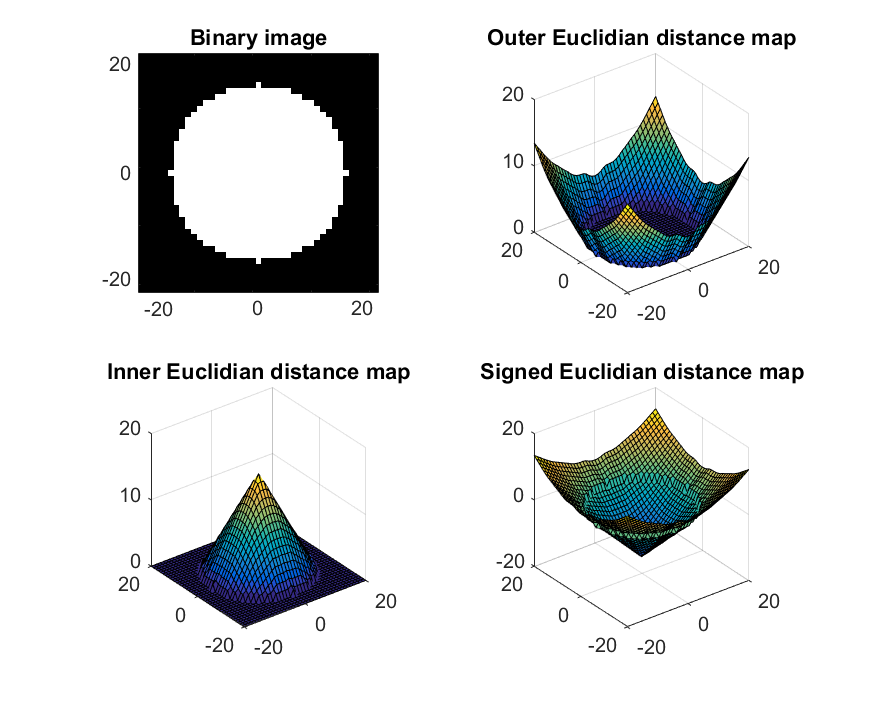
\includegraphics[width=0.8\linewidth]{img/distMap}
	\caption{Schematic representation of the distance map used for shape based averaging.}
	\label{fig:distMap}
\end{figure}

\lipsum[3] % place holder

\begin{figure}[h!]
	\centering
	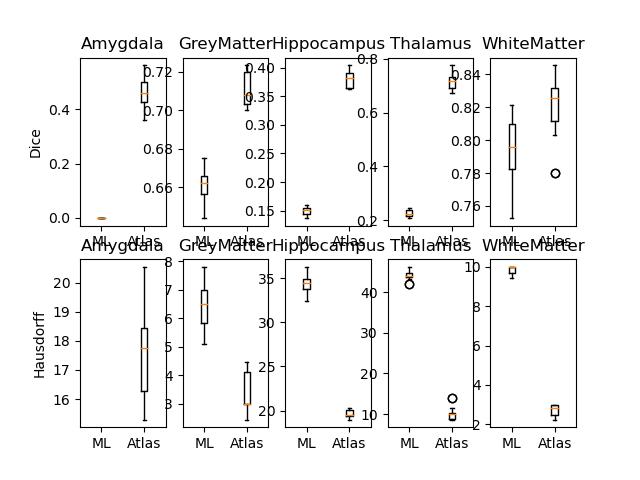
\includegraphics[width = .45 \textwidth]{img/boxplot}
	\caption{Boxplot graph}
	\label{fig:boxplot}
\end{figure}
\section*{Discussion}
The random forest parameters optimization could have been performed using a design of experiment instead. But this work focused more on the implementation of atlas-based segmentation methods.

The four atlas-based segmentation perform better with small brain parts, such as the amygdala, hippocampus and thalamus. This can be explained due to their relative static position and low distortion. 

For machine learning segmentation, grey and white matter have better results as atlas-based ones. Machine learning is able to interpret the subtle geometrical changes of those. This is clearly visible in the figure \ref{fig:compareGreyMatter}.

\begin{figure}[h!]
	\centering
	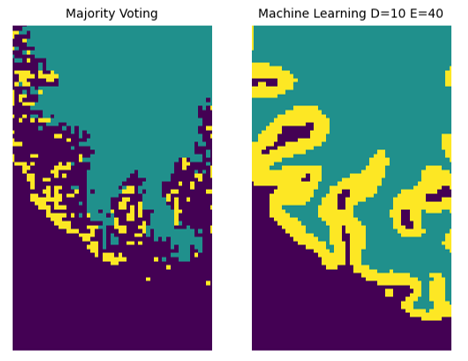
\includegraphics[width=.88\linewidth]{img/compareGreyMatter}
	\caption{Comparison between majority voting and machine learning segmentation for grey (yellow) and white matter (cyan).}
	\label{fig:compareGreyMatter}
\end{figure}

When comparing all four atlas-based segmentation algorithms, there is no major difference between majority voting, global weighted voting and shape based averaging. Local weighted voting significantly improves with grey and white matter, as seen in the results. The figure \ref{fig:compareSegmentationSlice} shows this case precisely. The edges of white matter and the grey matter are much more realistic and complete for the global weighted voting segmentation. The other three segmentations are very sparse at the frontier between grey and white matter.

\begin{figure}[h!]
	\centering
	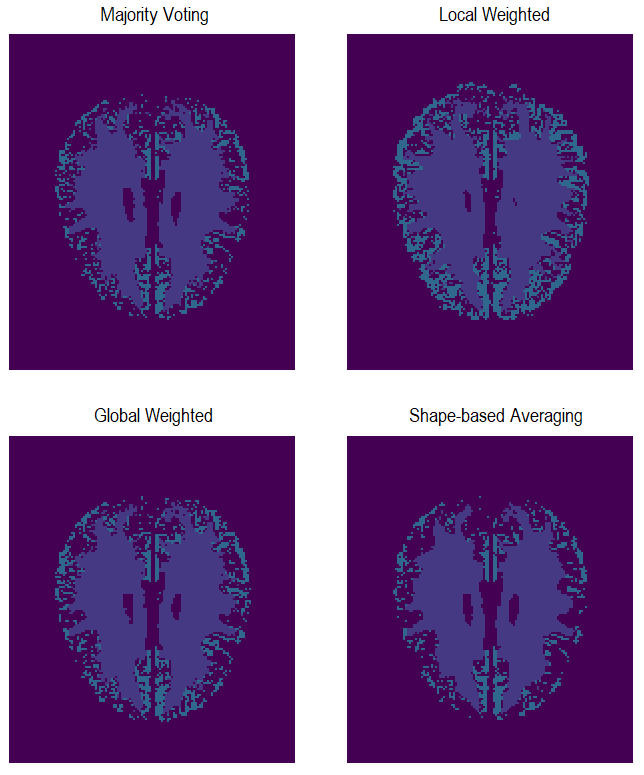
\includegraphics[width=.88\linewidth]{img/compareSegmentationSlice}
	\caption{Comparison between all 4 atlas-based segmentations for grey (cyan) and white matter (blue).}
	\label{fig:compareSegmentationSlice}
\end{figure}

Overall, the best performing algorithm of all those tested is the local weighted voting segmentation. The amygdala, hippocampus and thalamus have similar score as the other three atlas-based methods. The grey and white matter have a score close to the one with machine learning segmentation.
\lipsum[4] % place holder
\begin{thebibliography}{00}
\bibitem{b1} M. Young, The Technical Writer's Handbook. Mill Valley, CA: University Science, 1989. % place holder

\bibitem{b2} \color{red} X. Artaechevarria, A. Munoz-Barrutia and C. O. de Solorzano, "Combination strategies in multi-atlas image segmentation: Application to brain MR data", IEEE Trans. Med. Imag., vol. 28, no. 8, pp. 1266-1277, Aug. 2009.
\end{thebibliography}

\end{document}
